\section{Lecture 3: Instruction pipelining}
The idea is to divide the workload into different stages, so that we don't have to wait for an instruction to complete before we fetch the next one.

The typical pipeline has \textbf{six} stages: \\
1. Fetch Instruction (FI): Fetch the instruction.\\
2. Decode Instruction (DI): Determine the op-code and the operand specifiers.\\
3. Calculate Operands (CO): Calculate the effective addresses.\\
4. Fetch Operands (FO): Fetch the operands.\\
5. Execute Instruction (EI): perform the operation.\\
6. Write Operand (WO): store the result in memory.\\

The ideal case gives us a speed-up of six times. But in practice we have some problems.

In general, a larger number of stages gives better performance. \\
However, a large number also increases the complexity. We have to  move a lot of information between stages, and synchronize the stages. We call the problems that occur \textbf{Pipeline Hazards}.

\subsection{Pipeline hazards}
There are different kinds of pipeline hazards, first we have the case with dependency, A pipeline hazard occurs when the pipeline, or some portion of the pipeline, must stall because conditions do not permit continued execution. Such a pipe- line stall is also referred to as a pipeline bubble. There are three types of hazards: resource, data, and control. \\

\subsubsection{Structural (resource) hazards}
A \textbf{Resource hazards} resource hazard occurs when two (or more) instructions that are already in the pipeline need the same resource. The result is that the instructions must be executed in serial rather than parallel for a portion of the pipeline. A resource hazard is sometime referred to as a structural hazard.

\subsubsection{Data hazards}
A \textbf{Data Hazard} is when two instructions in a program are to be executed in sequence and both access a particular memory or register operand. If the two instructions are executed in strict sequence, no problem occurs. However, if the instructions are executed in a pipeline, then it is possible for the operand value to be updated in such a way as to produce a different result than would occur with strict sequential execution.

There are three types of data hazards: \\
• Read after write (RAW), or true dependency: An instruction modifies a reg- ister or memory location and a succeeding instruction reads the data in that memory or register location. A hazard occurs if the read takes place before the write operation is complete. \\
• Write after read(WAR), or antidependency: Aninstructionreadsaregisteror memory location and a succeeding instruction writes to the location. A hazard occurs if the write operation completes before the read operation takes place. \\
• Write after write (WAW), or output dependency: Two instructions both write to the same location. A hazard occurs if the write operations take place in the reverse order of the intended sequence. \\

We can handle this by using a technique called forwarding (bypassing). This works in the following way: \\
The ALU passes its result back into a MUX. If this detects that the value have been updated and not yet written back into the main memory, the value from the ALU will be used instead of the value we fetched from the memory as can be seen in figure \ref{fig:bypassing}.

\begin{figure}[H]
	\centering
	\scalebox{0.342}{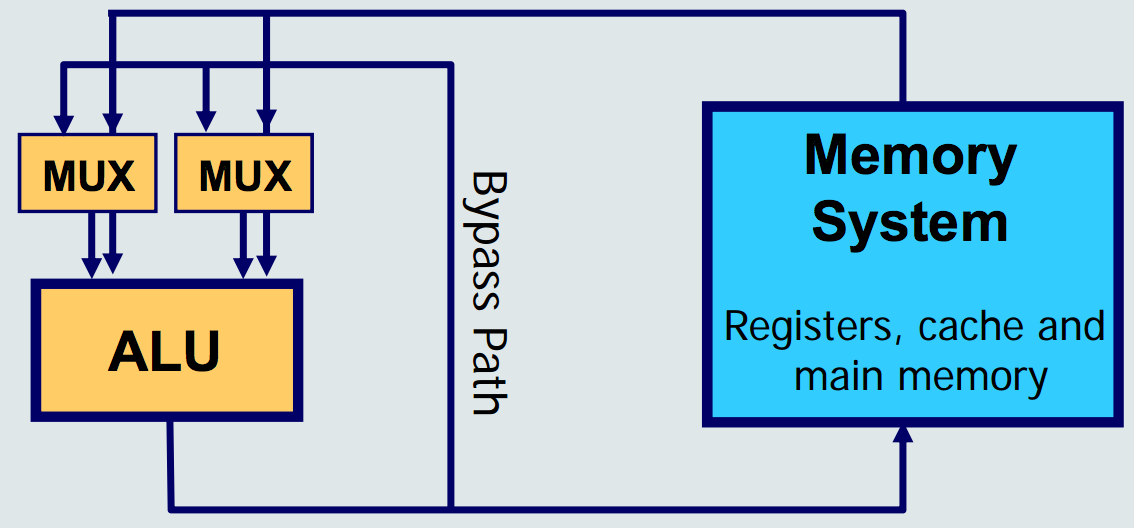
\includegraphics{img/bypassing.png}}
	\caption{The ALU passes its calculated value back into a MUX.}
	\label{fig:bypassing}
\end{figure}

\subsubsection{Control hazards}
A \textbf{control hazard}, also known as a branch hazard, occurs when the pipeline makes the wrong decision on a branch prediction and therefore brings instructions into the pipeline that must subsequently be discarded as seen in figure \ref{fig:control-hazard}.

\begin{figure}[H]
	\centering
	\scalebox{0.342}{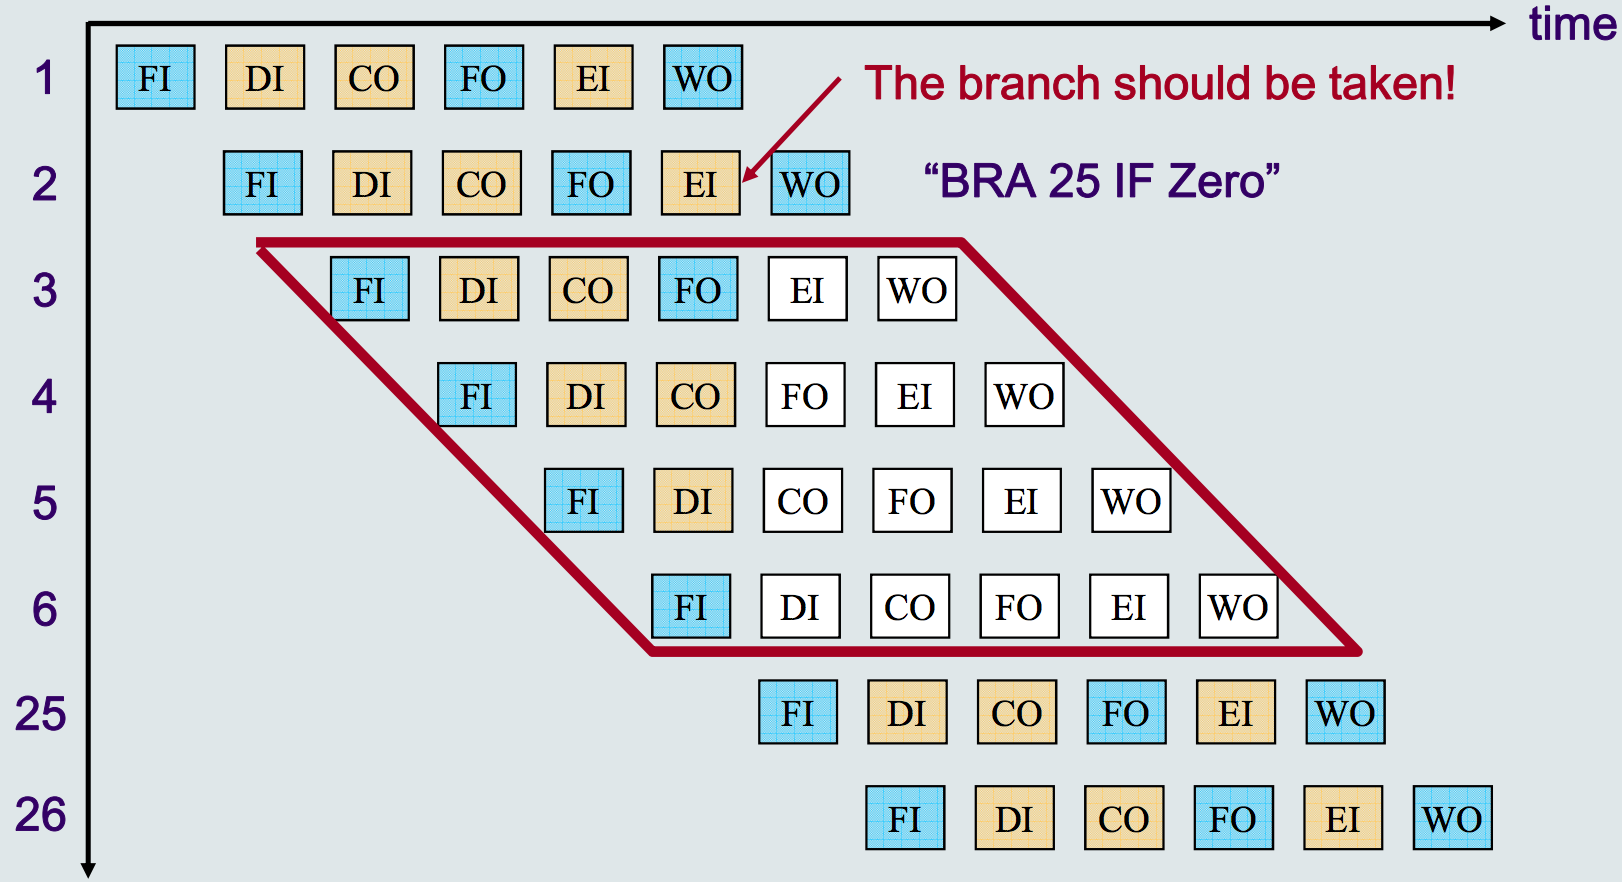
\includegraphics{img/control-hazard.png}}
	\caption{Control hazards.}
	\label{fig:control-hazard}
\end{figure}


\subsection{Branch handling}
There are different ways of handling branches. \\

\subsubsection{Stop the pipeline}
We can stall all the next instructions until the current branch reaches its final stage and we know what to do, this is expensive due to that 20-35\% of the things instructions executed are executed as branches.

\subsubsection{Multiple streams}
Implement hardware resources so that we can execute both alternatives in parallel, there are two problems with this though:
\begin{enumerate}
\item With multiple pipelines there are contention delays for access to the registers and to memory. \\
\item Additional branch instructions may enter the pipeline (either stream) before the original branch decision is resolved. Each such instruction needs an addi- tional stream.
\end{enumerate}

\subsubsection{Pre-fetch branch target}
When a conditional branch is recognized, the target of the branch is prefetched, in addition to the instruction following the branch. This target is then saved until the branch instruction is executed. If the branch is taken, the target has already been prefetched.

\subsubsection{Loop buffer}
A loop buffer is a small, very-high-speed memory maintained by the instruction fetch stage of the pipeline and containing the n most recently fetched instructions, in sequence. If a branch is to be taken, the hardware first checks whether the branch target is within the buffer. If so, the next instruction is fetched from the buffer. The loop buffer has three benefits:
\begin{enumerate}
\item With the use of prefetching, the loop buffer will contain some instruction sequentially ahead of the current instruction fetch address. Thus, instructions fetched in sequence will be available without the usual memory access time. 
\item If a branch occurs to a target just a few locations ahead of the address of the branch instruction, the target will already be in the buffer. This is use- ful for the rather common occurrence of IF–THEN and IF–THEN–ELSE sequences.
\item This strategy is particularly well suited to dealing with loops, or iterations; hence the name loop buffer. If the loop buffer is large enough to contain all the instructions in a loop, then those instructions need to be fetched from memory only once, for the first iteration. For subsequent iterations, all the needed instructions are already in the buffer.
\end{enumerate}

If the buffer contains 256 bytes, and byte addressing is used, then the least significant 8 bits are used to index the buffer. The remaining most significant bits are checked to determine if the branch target lies within the environment captured by the buffer.

\subsubsection{Delayed branch}
Re-arrange the instructions so that branching occur later than originally specified. This is a software solution.

\subsection{Branch prediction}
Various techniques can be used to predict whether a branch will be taken. Among the more common are the following:

\begin{itemize}
\item Predict never taken.
\item Predict always taken.
\item Predict by opcode.
\item Taken/not taken switch.
\item Branch history table
\end{itemize}



\subsubsection{Static Branch Prediction}
\textbf{Predict always taken} and \textbf{Predict never taken} those two either always predict the jump and fetches the next instruction or never does this respectively.

\textbf{Predict by opcode} branches based on the operation, this can be useful because some operations are more likely to result in a jump than others. For example: \\
\begin{itemize}
\item BNZ (Branch if the result is Not Zero).
\item BEZ (Branch if the result equals Zero)
\end{itemize}
\subsubsection{Dynamic Branch Prediction}
Here we branch based on the branch history, we can store information regarding branches in a branch-history table so that we more accurately can predict the branch outcome.

\subsubsection{Bimodal Prediction}
We want to use a 2-bit \underline{saturating counter} to predict the most common direction, where the first bit indicated the prediction. \\

Branches that doesn't take the branch will decrement the counter, and branches that takes the branch will increment it.
\textbf{This makes it possible to tolerate a branch going in the wrong direction one time}.

\begin{figure}[H]
	\centering
	\scalebox{0.342}{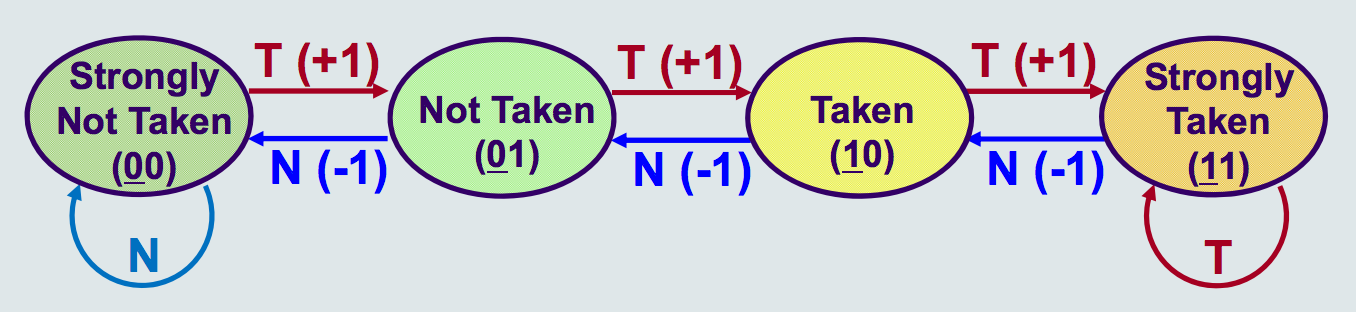
\includegraphics{img/bimodal-prediction.png}}
	\caption{Bimodal prediction using a 2-bit counter, much like a state diagram.}
	\label{fig:bimodal-prediction}
\end{figure}
